\lfoot{Autor: Raphael Simek}
\subsubsection{Motorwirkungsgrad}
\label{subsec:motorwirkungsgrad}

\textbf{Einführung\newline}
Es wurden Überlegungen in die Richtung des Motorwirkungsgrades angestellt, um basierend auf den eingeholten Informationen einen Schaltvorschlag errechnen zu können. Ein Schaltvorschlag ist ein Hinweis für einen Nutzer, worauf und wann dieser Schalten könnte. Ein derartiger Vorschlag bietet Optionen bezüglich der Visualisierung und des angestrebten Effekts (siehe 3.3 Schaltvorschlag). Für das weitere Verständnis sind allerdings einige Grundlagen von besonderer Relevanz:
Ein Teil des Projektes möchte dem Fahrer Informationen zu einem möglichst idealen Schaltzeitpunkt zur Verfügung stellen. Dabei spielt der Wirkungsgrad hinsichtlich des Spritverbrauchs eine entscheidende Rolle. Ein niedriger Spritverbrauch (Wirkungsgrad) bedeutet deshalb nicht, dass der \ce{CO2}-Ausstoß niedrig ist. Der Katalysator hat einen eigenen Wirkungsgrad, welcher für diese Rechnung einbezogen werden muss. Für das Diplomprojekt beschlossen wir den Motorwirkungsgrad in den Fokus zu setzen.

\begin{wrapfigure}{r}{0.6\textwidth}\centering
    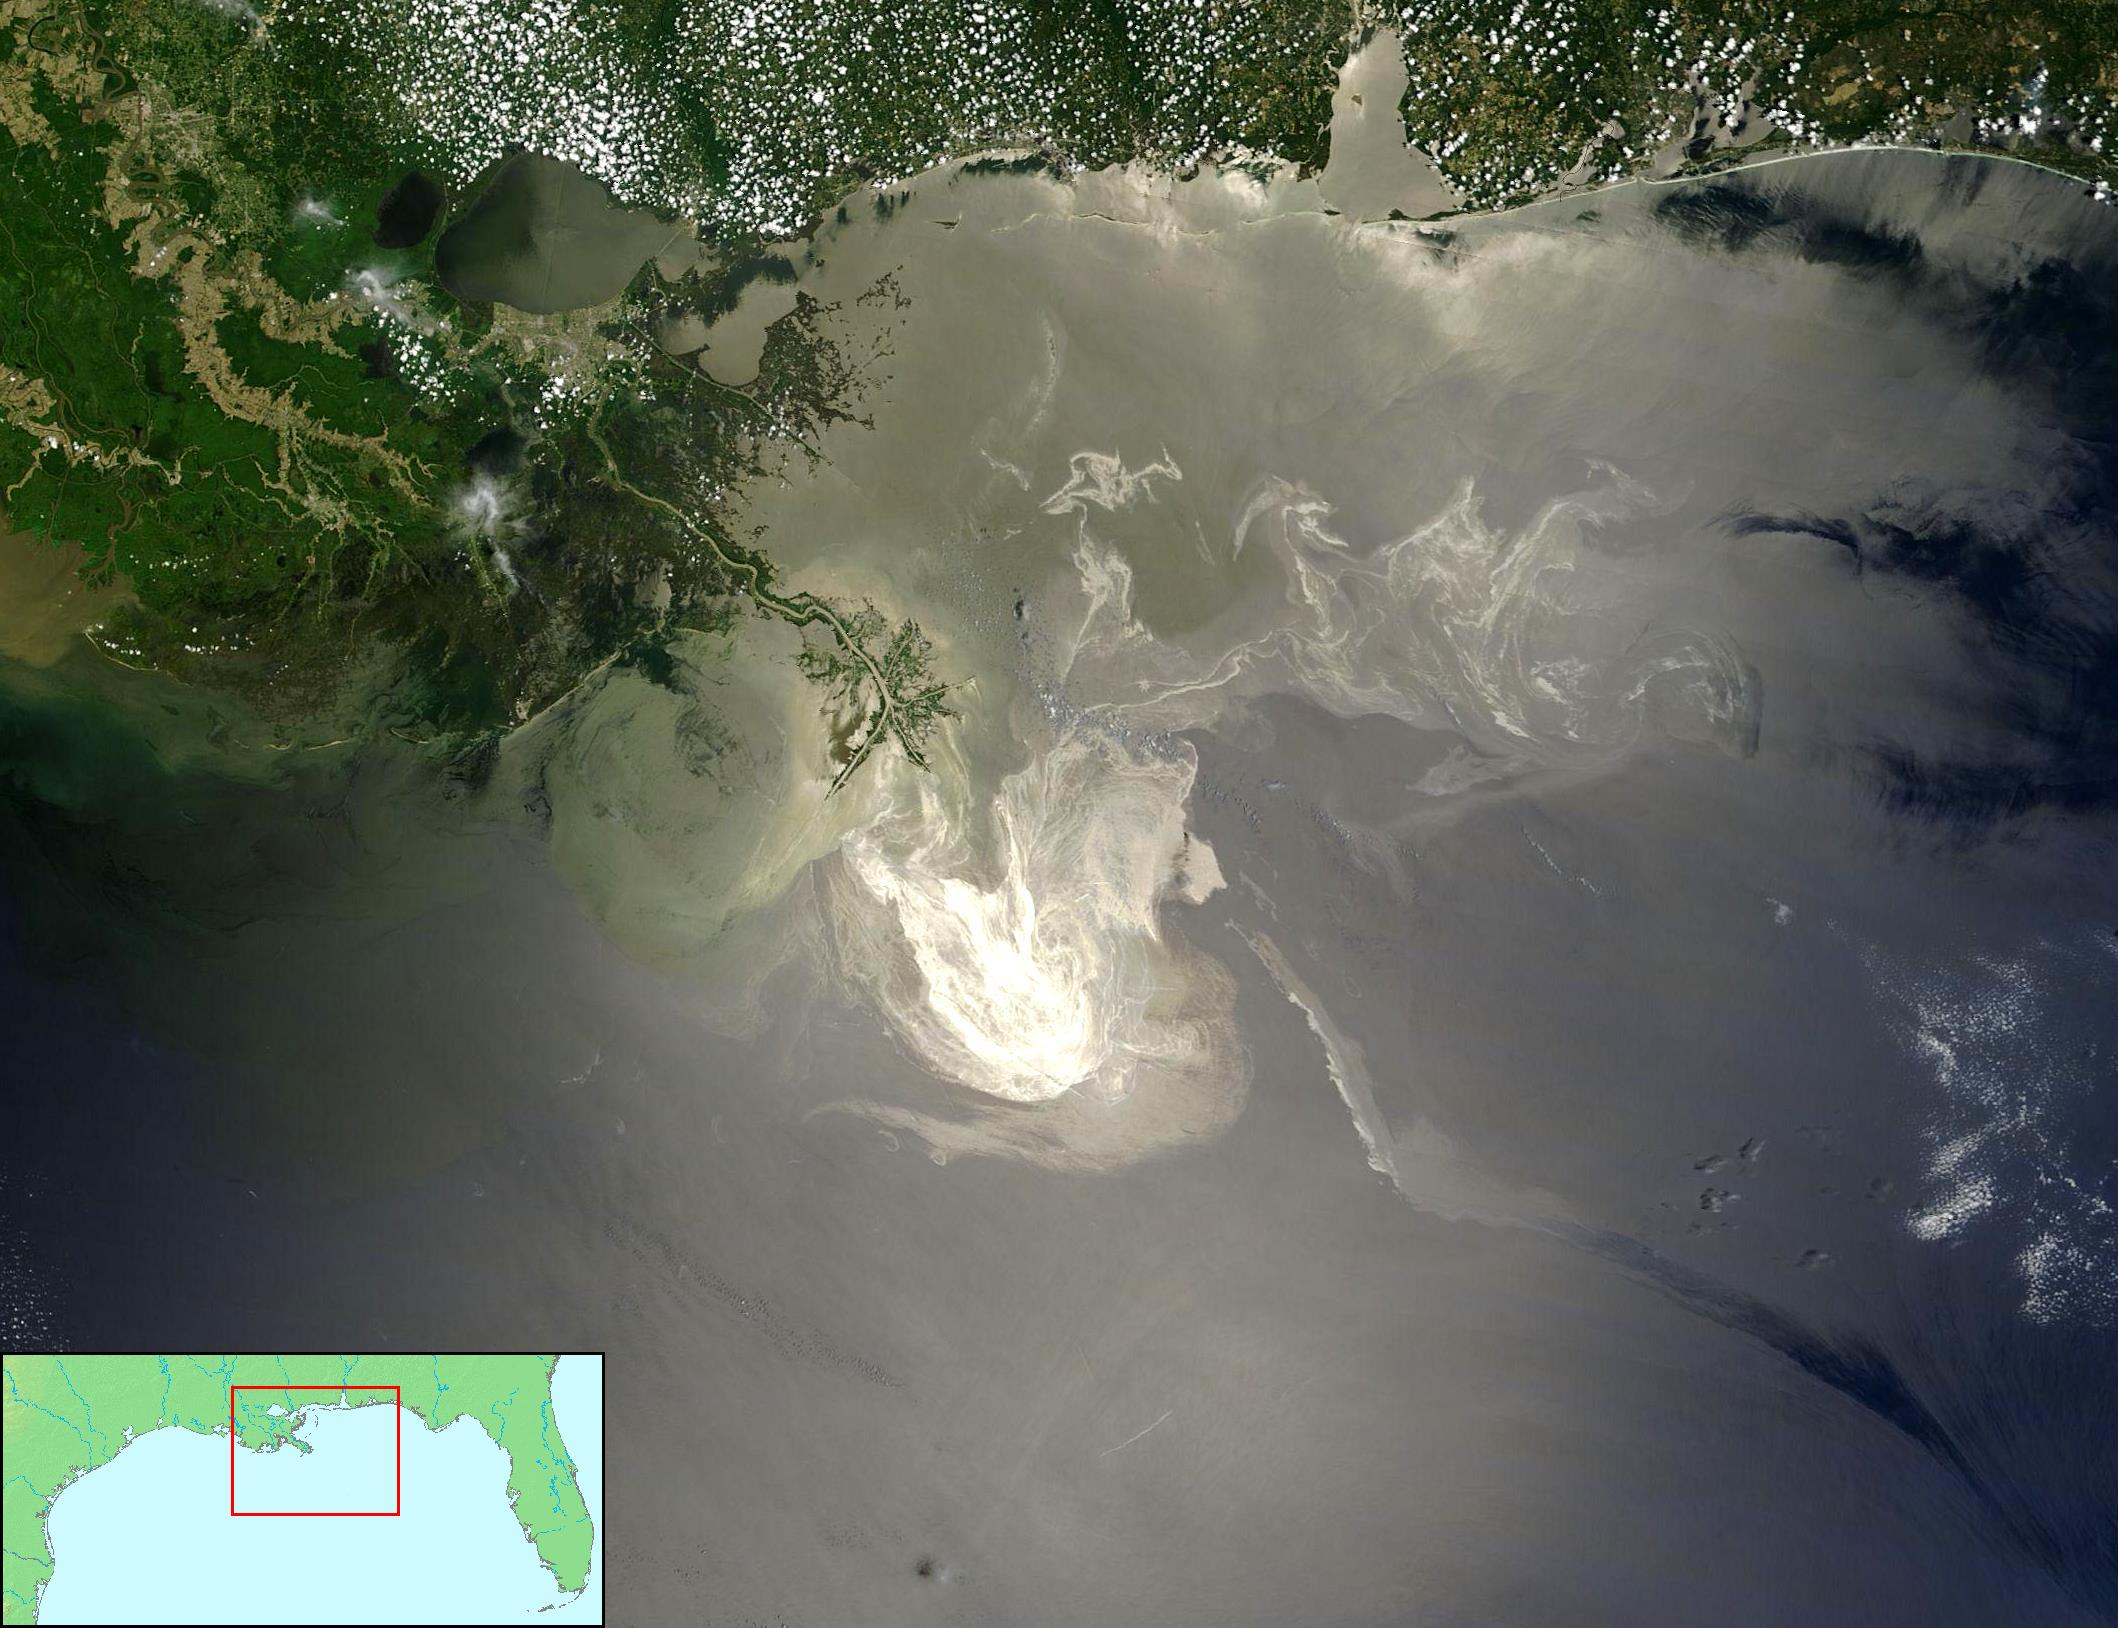
\includegraphics[width=0.6\textwidth]{images/bpOilSpillSatelite}
    \caption{1 Monat nach der Explosion \cite{SIMR.CH2-motorwirkungsgrad.bpOilSpillSatelite}} \label{Fig:imgBPOilSpill}
\end{wrapfigure}
Eine effiziente Fahrweise ist besonders in Bezug auf die immer restriktiveren Emissionsbestimmungen und die häufig hohen Kraftstoffpreise von Interesse für Autofahrer. Zusätzlich sind fossile Brennstoffe, nicht erneuerbare Ressourcen. Genau deshalb ist es besonders wichtig sparsam und ökonomisch mit der bald erschöpften Ressource Erdöl umzugehen. 
Denn die Öl-Förderung erzeugt schon heute Naturkatastrophen und Umweltverschmutzung und wird immer schwerer zu erlangen.
Naturkatastrophen wie BP's \textit{Deepwater Horizon} Ölpest aus dem Jahre 2010 \cite{SIMR.CH2-motorwirkungsgrad.BPSpillGeneral}, bei welcher 3 Jahre nach der Explosion weiterhin Rekordzahlen von Delphinen und Wasserschildkröten starben \cite{SIMR.CH2-motorwirkungsgrad.BPSpillDeaths}. 

\textbf{Zielsetzung\newline}
Geplant wurde ein möglichst kraftstoffeffizienter Schaltvorschlag.
Die Formel \textit{Kraftstoffmenge = Strecke * Verbrauch} gibt einem Autofahrer 2 Optionen, seinen Kraftstoffverbrauch zu minimieren. Option 1 wäre weniger zu fahren, Option 2 verbrauchsärmer zu fahren. Hier steht die 2. Option im Fokus. 
Zur weiteren Erläuterung, wie der Schaltvorgang in diesem Projekt umgesetzt wurde, soll hier ein kurzer Überblick über die Funktion eines 4-Takt Verbrennungsmotors gegeben werden. Ein Takt ist ein Kolbenhub, also eine Auf- oder Abwärtsbewegung des Kolbens. Der Kreisprozess (siehe Carnot-Prozess) von 4 Takten dreht sich die Kurbenwelle folglich zweimal.

\paragraph{Ansaugen}
Der Kolben bewegt sich in diesem Takt nach unten. Das Einlassventil wird geöffnet und Gas-/Luft-Gemisch gelangt in den Zylinder. Das vordefinierte Volumen oberhalb des Kolbens (Kompressionsvolumen) wird mit diesem Gemisch gefüllt.
\paragraph{Verdichten} 
Im 2. Takt treibt die Kurbelwelle den Kolben nach oben bis in seinen Totpunkt. Das Gas-Luft Gemisch wird in diesem Takt, bei geschlossenen Ventilen, verdichtet.
\paragraph{Explosion / Arbeitstakt}
In diesem Takt erfolgt die Explosion des Gas-Luft Gemisch in der Verbrennungskammer. Bei der Explosion vergrößert sich das Volumen oberhalb des Kolbens schlagartig um 50\% im Gegensatz zum 1. Takt. Diese schlagartige Volumenvergrößerung beschleunigt den Kolben und treibt die Kurbelwelle an, womit die Energie der Verbrennung in Rotationsenergie gewandelt wird. 
\paragraph{Ausstoß}
Das Auslassventil wird geöffnet und der Kolben drückt die, bei der Verbrennung entstandenen, Gase aus der Brennkammer heraus. In der Theorie treffen sich dabei Abgabe und Gas-Luft Gemisch gar nicht, was in der Praxis allerdings vorkommt \cite{SIMR.CH2-motorwirkungsgrad.4strokeEngine}.

\begin{figure}[!htb]\centering
	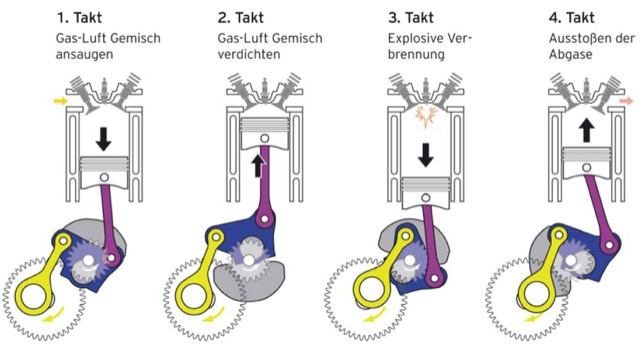
\includegraphics[width=0.8\textwidth]{images/viertaktMotorPrinzip}
	\caption{Prinzip eines 4-Takt Motors \cite{SIMR.CH2-motorwirkungsgrad.4strokeEngine}}\label{Fig:img4strokeEngine}
\end{figure}

Verlorene Energie bei der Verbrennung:\newline
direktes Zitat: \cite{SIMR.CH1-Fahrstil-Analyse.Motorkennfeld}
\textit{
\begin{itemize}
	\item \glqq Auspuff: 36\% ausgestoßene Wärme
	\item Durch Zylinderwände: 33\% Abwärme, Teil davon für die Heizung
	\item Motorreibung: Reibung verlangt der Motorbewegung 8\% der Gesamtenergie ab \grqq
\end{itemize}}
So bleiben im besten Falle 30\% über, die auf die Reifen übertragen werden. Diese 30\% sind zumeist nur unter Volllast erreichbar. Neue Piezopumpedüse (PPD) Diesel-Motoren schaffen im Optimalfall einen Wirkungsgrad von 45\%, das ist aber bei Verbrennungsmotoren das momentane Optimum \cite{SIMR.CH2-motorwirkungsgrad.maxWirkungsgrad}. Diese wenige Energie die der Motor, aus dem Tropfen Kraftstoff, der eingespritzt wird, erlangt, wird dann durch folgende Widerstände erneut geschwächt:\newline
direktes Zitat: \cite{SIMR.CH1-Fahrstil-Analyse.Motorkennfeld}
\textit{
\begin{itemize}
	\item \glqq Beschleunigungswiderstand: Das Beschleunigen eines Körpers braucht Energie. Die Energie wächst quadratisch mit der Geschwindigkeit, sie bleibt aber als \textit{kinetische Energie} in der Geschwindigkeit. 
	\item Steigungswiderstand: Nutzenergie wird beim Bergauffahren gebraucht. Sie bleibt als \textit{potenzielle Energie} gespeichert, welche Abgerufen wird, wenn wieder bergab gefahren wird.
	\item Rollreibung: Diese stellt sich jeder Bewegung in den Weg. Je nach Beschaffenheit der Straße und der Reifen reiben beide aneinander und erwärmen sich. Bei steigender Geschwindigkeit oder niedrigem Reifendruck steigt diese Reibung an.
	\item Luftwiderstand: Diese verdrückt mit zunehmender Geschwindigkeit mehr Energie. Weil bei doppelter Geschwindigkeit nicht nur doppelt so viel Luft verdrängt werden muss, sondern sie auch mit doppelter Geschwindigkeit aufprallt, wächst die bremsende Kraft quadratisch. 
	\item (Bremsen): Dieser Widerstand tritt nicht ständig auf, sondern hängt ausschließlich von seinem Fahrstil ab. Hierbei ist der häufige Wechsel von beschleunigen und bremsen gemeint, was so erneut einen quadratischen Widerstand darstellt.\grqq
\end{itemize}}

Alle diese Faktoren sind sehr stark vom eigenen Fahrstil abhängig, welcher dadurch auch den Verbrauch diktiert. Daraus folgt, dass versucht werden muss diese Widerstände durch möglichst effektives Fahren im Straßenverkehr so gering als möglich zu halten.

Zielsetzung ist es, dem Fahrer einen optimalen Schaltvorschlag zu machen und das Fahrzeug in möglichst hohem Motorwirkungsgrad zu halten. Das heißt, aus jedem Tropfen eingespritztem Kraftstoff möglichst viel Energie zu gewinnen. Deshalb wird bei diesem Ansatz auch bewusst dazu aufgefordert den Motor weitaus höher als bei einem konventionellen Schaltvorschlag zu drehen bzw. mit höherer Motorlast zu fahren.
 
Bordcomputer unterscheiden sich voneinander oft stark. Viele Autos bieten zum Zweck der Verbrauchsmessung nur eine Anzeige des Momentanverbrauchs, welcher wenig hilfreich ist. Anhand dieser Berechnungen kann man keine Schlüsse auf die Fahrweise ziehen. Einige glätten den Verbrauch auf einen Zeitraum, doch alle gemeinsam haben sie, dass die nicht ausreichend dokumentiert sind um faktische Rückschlüsse auf den Fahrstil treffen zu können.

\textbf{Bonanza-Effekt oder Torsionsschwingungen im Antriebsstrang\nextline}
Direktes Zitat: \cite{SIMR.CH2-motorwirkungsgrad.Motorschwingungen}
\textit{
\glqq Der Verkehr stockt und zwingt den Autofahrer zum Bremsen, er schaltet jedoch nicht in einen niedrigeren Gang. In solchen Fällen ist oftmals ein Brummen zu hören: Die Torsionsschwingung verursacht das unangenehme Geräusch. Sie tritt auf, da sich die Kurbelwelle bei Verbrennungsmotoren nie ganz gleichförmig dreht. Diese Drehschwingung belastet das Getriebe, im schlimmsten Fall leidet die Lebensdauer des Motors – er geht früher kaputt. Auch in anderen Antriebssträngen, die mit einem Verbrennungsmotor gekoppelt sind, kommt es zu dem unerwünschten Effekt – etwa in Schiffen oder Produktionsmaschinen. Grundsätzlich gibt es zwar Lösungen, um ihn ausgleichen. Da die Motoren jedoch immer effizienter werden, nehmen auch die Schwingungen zu – die bestehenden Ausgleichssysteme kommen an ihre Grenzen. Ein Beispiel: Beim PKW geht der Trend zu weniger Zylindern oder aber dazu, einzelne Zylinder zeitweise abzuschalten. Dies hat zur Folge, dass der Motor weniger rund läuft und vermehrt Torsionsschwingungen auftreten. Bei Schiffen entstehen sie, wenn im Hafen von Schweröl oder Dieselantrieb auf Gas umgeschaltet wird, um die Emissionen zu reduzieren.\grqq} 

Demnach ist es also wichtig die Torsionsschwingungen zu vermeiden. Diese Schwingungen treten am Stärksten in hohem Gang bei niedriger Drehzahl aber hoher Last auf. Diese Schwingungen sind konkret auf dem bei Abb. \ref{Fig:imgEngineVibrations} gezeigtem Motorkennfeld im oberen drittel des Drehmoments im Bereich von <1000rpm angesiedelt. Dieser Bereich ist nicht eingezeichnet, da in diesem Bereich massive Schwankungen des Motormoments auftreten. Dieser Bereich umfasst Motormomente, die das 3-fache der sonst üblichen Torsionsschwingungen übersteigen. Überdies produziert der Motor innerhalb dieses Bereiches kaum Leistung.

\begin{figure}[!htb]\centering
	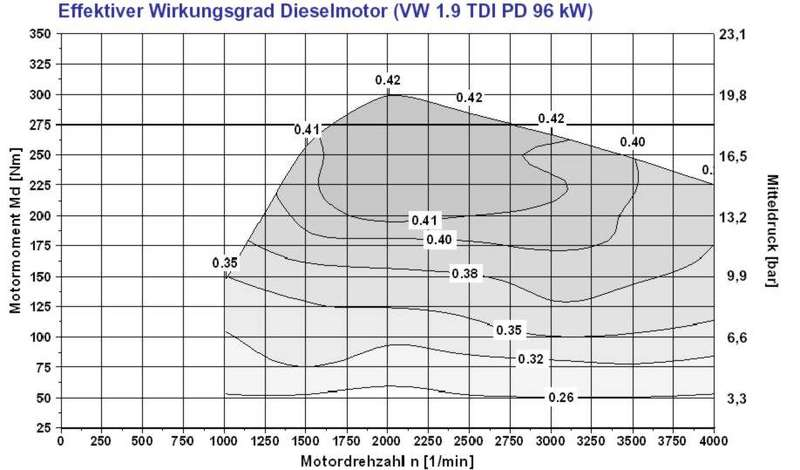
\includegraphics[width=0.8\textwidth]{images/poloMotorkennfeld}
	\caption{Motorkennfeld eines VW Polo 
	 \cite{SIMR.CH2-motorwirkungsgrad.SchwingungenMotorkennfeld}}\label{Fig:imgEngineVibrations}
\end{figure}

%move to the end
Das erlangte Grundwissen diente uns als Basis für die konkrete Implementierung des Schaltvorgangs.
In Zusammenarbeit mit Prof. Neuburger aus der Fahrzeugtechnik Abteilung des TGM wurden Kriterien für die Schaltvorschläge festgelegt. Ein Nutzer würde beispielsweise dazu aufgefordert werden bei Erreichen von 90\% des max. Drehmoments oder der maximalen Drehzahl, hochzuschalten. Ebenso würde ein Nutzer dazu aufgefordert werden herunterzuschalten, so dieser einen hohen Gang mit überdurchschnittlich niedriger Drehzahl fährt.

Zusammengefasst:
\begin{itemize}
	\item 90\% der max. Drehzahl oder Drehmoment --> hochschalten, wegen niedrigem Wirkungsgrad
	\item niedrige Drehzahl und hohe Last --> herunterschalten, wegen Verschleiß durch Motorschwingungen
\end{itemize}
Die genaue technische Umsetzung und Implementierung des Schaltvorschlags wird im Kapitel Schaltvorschlag \ref{subsec:schaltvorschlag}.

\clearpage % DO NOT REMOVE